\title{Homework 4}
\author{Crist\'obal Armaza, Chris Silvia}
\date{\today}

\documentclass[11pt]{article}
\usepackage[letterpaper,left=2.2cm,right=2.2cm,top=2.2cm,bottom=2.5cm]{geometry}
\usepackage{graphicx}
\usepackage{hyperref}
\DeclareGraphicsExtensions{.bmp,.png,.jpg,.pdf}
\usepackage{amsmath}
\usepackage{courier}
\usepackage{natbib}
\linespread{1.2}

\newcommand{\Ma}{\text{Ma}}
\newcommand{\Rey}{\text{Re}}
\newcommand{\ind}[4]{{#1}^{#2}_{#3,#4}}

\begin{document}
\maketitle

\section*{Organization}


\section{Analytical Equations}

\subsection{Navier-Stokes for an incompressible fluid}

We want to solve the continuity equation
\begin{equation}
\frac{\partial \rho}{\partial t} + \frac{\partial}{\partial x_k}\left(\rho u_k\right) = 0,
\end{equation}
and the momentum equation
\begin{equation}
\frac{\partial}{\partial t}\left(\rho u_i\right) + \frac{\partial}{\partial x_k}\left(\rho u_k u_i\right) = -\frac{\partial p}{\partial x_i} + \frac{\partial}{\partial x_k}\left[\mu\left(\frac{\partial u_i}{\partial x_k} + \frac{\partial u_k}{\partial x_i}- \frac{2}{3}\delta_{ik}\frac{\partial u_l}{\partial x_l}\right)\right],
\end{equation}
where we will assume that the fluid is incompressible, i.e. $D\rho/Dt = 0$. This implies the solenoidal condition 
\begin{equation}
\frac{\partial u_k}{\partial x_k} = 0,
\end{equation}
which, in turn, helps simplify the momentum equation, giving
\begin{equation}
\frac{\partial u_i}{\partial t} + \frac{\partial}{\partial x_k}\left(u_k u_i\right) = -\frac{1}{\rho}\frac{\partial p}{\partial x_i} + \frac{\mu}{\rho}\frac{\partial^2 u_i}{\partial x_k \partial x_k}.
\end{equation}
In dimensionless form, the continuity equation remains the same, while the momentum equation is
\begin{equation}
\frac{\partial u_i}{\partial t} + \frac{\partial}{\partial x_k}\left(u_k u_i\right) = -\frac{\partial p}{\partial x_i} + \frac{1}{\Rey}\frac{\partial^2 u_i}{\partial x_k \partial x_k}.
\end{equation}

\subsection{2-D Equations in Cartesian Equations}

Introduce the Cartesian system $x_k = (x, y)$ and the vector $u_i = (u, v)$. In dimensionless form, we want to solve the initial-value problem 
\begin{align}
\frac{\partial u}{\partial x} + \frac{\partial v}{\partial y} &= 0\\
\frac{\partial u}{\partial t} + \frac{\partial u^2}{\partial x} + \frac{\partial (uv)}{\partial y} &= -\frac{\partial p}{\partial x} + \frac{1}{\Rey}\left( \frac{\partial^2 u}{\partial x^2} + \frac{\partial^2 u}{\partial y^2} \right)\\
\frac{\partial v}{\partial t} + \frac{\partial (vu)}{\partial x} + \frac{\partial v^2}{\partial y} &= -\frac{\partial p}{\partial y} + \frac{1}{\Rey}\left( \frac{\partial^2 v}{\partial x^2} + \frac{\partial^2 v}{\partial y^2} \right)
\end{align}
with given boundary conditions. These are three equations for the three variables $p(x,y,t)$, $u(x,y,t)$ and $v(x,y,t)$.

\section{Numerics}

Following the instructions of this assignment, we treat spatial and time discretization in different ways, the details of which are given below.

\subsection{Spatial Discretization}

First, we discretize the domain into a rectangular mesh of $n_x\times n_y$ cells, labeled $(i,j)$. The cells will be regular, having a volume $\Delta x\,\Delta y$. On each cell, we store the pressure at the center, $p(n,i,j) = \ind{p}{n}{i}{j}$, the $x-$velocity at the left face, $u(n,i,j) = \ind{u}{n}{i-1/2}{j}$, and the $y-$velocity at the bottom face, $v(n,i,j) = \ind{v}{n}{i}{j-1/2}$. Figure \ref{staggering} shows the indexation in our code. In this finite volume method scheme, the control volume used for all the three equations is different. In what follows we provide the detailed formulas for each equation. All of these expressions involve quantities evaluated at the same time step, so we omit the subscript $n$. 

\begin{center}
\begin{figure}[ht!]
\begin{minipage}{12cm}\label{staggering}
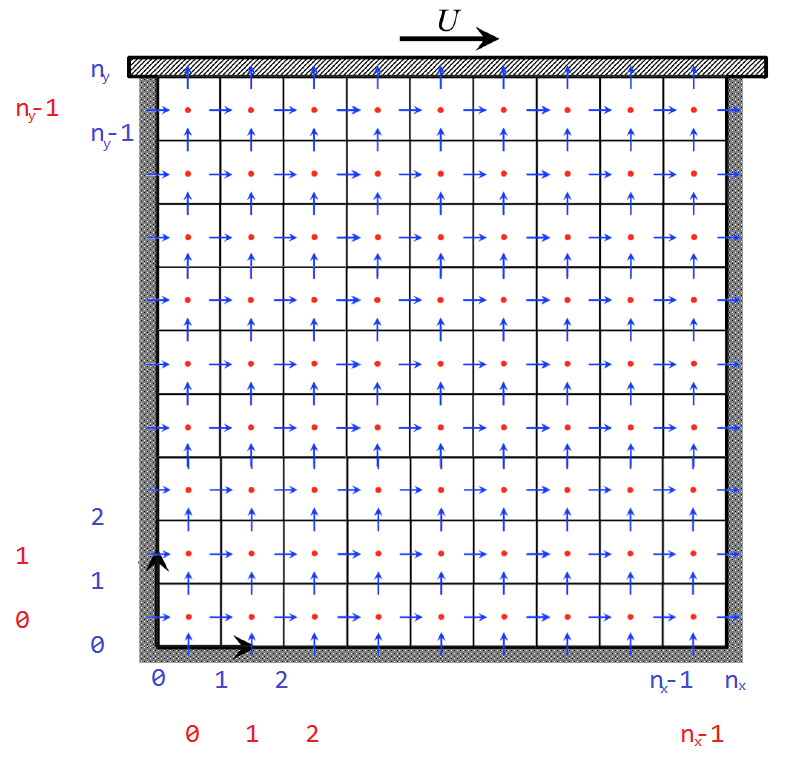
\includegraphics[width=12cm]{staggering.png}
\end{minipage}
\caption{Staggering in our code. (Figure adapted from the one provided for this assignment.)}
\end{figure}
\end{center}

\subsubsection{Continuity Equation}

We will not be explicitly solving the continuity equation. Instead, we will \emph{ensure} that the solenoidal condition is satisfied at every time step, the details of which will be given below. For future reference, we exhibit the approximation for the divergence of the velocity. For this, the control volume is centered at the center of the cell, so we label it as $(i,j)$. The discretization is
\begin{equation}\label{contin}
(\nabla\cdot\mathbf u)_{i,j} = \frac{u_{i+1/2,j} - u_{i-1/2,j}}{\Delta x} + \frac{v_{i,j+1/2} - v_{i,j-1/2}}{\Delta y},
\end{equation}
for $i = 0,\hdots,n_x-1$, $j = 0,\hdots,n_y-1$. These expressions are formally second-order accurate. Same thing with the momentum equations below. 


\subsubsection{\texorpdfstring{$x-$}mmomentum Equation}

The control volume is centered at the left face of the cell, so we label it as $(i-1/2, j)$. Ignoring the pressure term for now, the discretization is
\begin{align}\nonumber
\left.\frac{\partial u}{\partial t}\right|_{i-1/2,j} 
&= -  \frac{u_{i,j}\,u_{i,j} - u_{i-1,j}\,u_{i-1,j}}{\Delta x}\\\nonumber
&\quad - \frac{u_{i-1/2,j+1/2}\,v_{i-1/2,j+1/2} - u_{i-1/2,j-1/2}\,v_{i-1/2,j-1/2}}{\Delta y}\\
&\quad + \frac{1}{\Rey}\frac{u_{i+1/2,j} - 2u_{i-1/2,j} + u_{i-3/2,j}}{\Delta x^2} 
+ \frac{1}{\Rey}\frac{u_{i-1/2,j+1} - 2u_{i-1/2,j} + u_{i-1/2,j-1}}{\Delta y^2}.\label{dudt}
\end{align}
This is valid for $i = 1,\hdots,n_x-1$, $i = j,\hdots,n_y-2$.

\subsubsection{\texorpdfstring{$y-$}mmomentum Equation}

The control volume is centered at the bottom face of the cell, so we label it as $(i,j-1/2)$. Ignoring the pressure term for now, the discretization is
\begin{align}\nonumber
\left.\frac{\partial v}{\partial t}\right|_{i,j-1/2} &= - \frac{v_{i+1/2,j-1/2}\,u_{i+1/2,j-1/2} - v_{i-1/2,j-1/2}\,u_{i-1/2,j-1/2}}{\Delta x}\\\nonumber
&\quad - \frac{v_{i,j}\,v_{i,j} - v_{i,j-1}\,v_{i,j-1}}{\Delta y}\\
&\quad + \frac{1}{\Rey}\frac{v_{i+1,j-1/2} - 2v_{i,j-1/2} + v_{i-1,j-1/2}}{\Delta x^2}
+ \frac{1}{\Rey}\frac{ v_{i,j+1/2} - 2v_{i,j-1/2} + v_{i,j-3/2} }{\Delta y^2}.\label{dvdt}
\end{align}
In the two previous equations, the following definitions must be introduced,
\begin{align}
u_{i,j} &= \frac{u_{i+1/2,j} + u_{i-1/2,j}}{2},\\
v_{i,j} &= \frac{v_{i,j+1/2} + v_{i,j-1/2}}{2},\\
u_{i-1/2,j-1/2} &= \frac{u_{i-1/2,j} + u_{i-1/2,j-1}}{2},\\
v_{i-1/2,j-1/2} &= \frac{v_{i,j-1/2} + v_{i-1,j-1/2}}{2}.
\end{align}
This is valid for $i = 1,\hdots,n_x-2$, $i = j,\hdots,n_y-1$.

\subsection{Time discretization}

For this task, we use a simplified version of the scheme proposed by Kim and Moin (1985), consisting of three steps.

\textbf{Step 1.} Advance the momentum equation without the pressure term using an intermediate time step
\begin{align}
\ind{u}{\star}{i-1/2}{j} &= \ind{u}{n}{i-1/2}{j} + \Delta t\,\left.\frac{\partial u}{\partial t}\right|_{i-1/2,j},\\
\ind{v}{\star}{i}{j-1/2} &= \ind{v}{n}{i}{j-1/2} + \Delta t\,\left.\frac{\partial v}{\partial t}\right|_{i,j-1/2}.
\end{align}
The last term in both equations is given by Eqn. \eqref{dudt} and \eqref{dvdt}, respectively. 

\textbf{Step 2.} Given the advanced velocity $\mathbf u^\star$, obtain the advanced pressure $\ind{p}{n+1}{i}{j}$ from the Poisson equation
\begin{equation}
\nabla\cdot(\nabla p^{n+1})_{i,j} = \frac{1}{\Delta t}\left(\nabla\cdot\mathbf u^\star\right)_{i,j},
\end{equation}
where 
\begin{equation}
\left(\nabla\cdot\mathbf u^\star\right)_{i,j} = \frac{u^\star_{i+1/2,j} - u^\star_{i-1/2,j}}{\Delta x} + \frac{v^\star_{i,j+1/2} - v^\star_{i,j-1/2}}{\Delta y}.
\end{equation}
The resolution of the Poisson equation is discussed later in an independent section.

\textbf{Step 3.} Given $\ind{p}{n+1}{i}{j}$, add the pressure term to the advanced velocity,
\begin{align}
\ind{u}{n+1}{i-1/2}{j} &= \ind{u}{\star}{i-1/2}{j} - \frac{\Delta t}{\Delta x}\left(\ind{p}{n+1}{i}{j} - \ind{p}{n+1}{i-1}{j} \right),\\
\ind{v}{n+1}{i}{j-1/2} &= \ind{v}{\star}{i}{j-1/2} - \frac{\Delta t}{\Delta y}\left(\ind{p}{n+1}{i}{j} - \ind{p}{n+1}{i}{j-1} \right).
\end{align}

\subsection{System To Be Solved}

From the setup above, inside of the domain we have $n_x\times n_y$ pressure unknowns, $(n_x - 1)\times n_y$ $x-$velocity unknowns, and $n_x\times(n_y - 1)$ $y-$velocity unknowns. Provided boundary conditions for the $2n_y$ $x-$velocities at the left and right walls, and $2n_x$ $y-$velocities at the top and bottom walls, plus compatible boundary conditions for the pressure at the walls, the system can be solved.

\section{Boundary Conditions}

We are interested in solving the 2D lid-driven cavity flow. Conveniently enough, our setup requires simple boundary conditions for the normal velocities at the walls,
\begin{align}
u_{-1/2,j} = u_{n_x - 1/2,j} &= 0;\quad j = 0,\hdots,n_y-1,\\
v_{i,-1/2} = v_{i,n_y - 1/2} &= 0;\quad i = 0,\hdots,n_x-1.
\end{align}
The actual difficulty of boundary conditions arises when noticing that one of the viscous terms in Eqns. \eqref{dudt} and \eqref{dvdt} (the one consisting of the second derivative along the normal to the wall) requires evaluating the tangential velocity \emph{inside} of the wall (i.e., outside of the domain). For these points, the corresponding viscous term must be replaced by an asymmetric derivative. Following the example provided in the assignment, we obtain
\begin{align}
\left.\frac{\partial^2 v}{\partial x^2}\right|_{0,j-1/2} 
&= \frac{1}{\Delta x^2}\left( v_{1,j-1/2} - 3v_{0,j-1/2} + 2v_{lw} \right),\\
\left.\frac{\partial^2 v}{\partial x^2}\right|_{n_x-1,j-1/2}
&= \frac{1}{\Delta x^2}\left( 2v_{rw} - 3v_{n_x-1,j-1/2} + v_{n_x-2,j-1/2} \right)
\end{align}
for the left and right walls, respectively, where $j=1,\hdots n_y-1$, and 
\begin{align}
\left.\frac{\partial^2 u}{\partial y^2}\right|_{i-1/2,0}
&= \frac{1}{\Delta y^2}\left( u_{i-1/2,1} - 3u_{i-1/2,0} + 2u_{bw} \right),\\
\left.\frac{\partial^2 u}{\partial y^2}\right|_{i-1/2,n_y-1} 
&= \frac{1}{\Delta y^2}\left( 2u_{tw} - 3u_{i-1/2,n_y-1} + u_{i-1/2,n_y-2} \right)
\end{align}
for the bottom and top walls, respectively, where $i = 1,\hdots, n_x-1$. Here,
\begin{equation}
v_{lw} = 0;\qquad v_{rw} = 0;\qquad u_{bw} = 0;\qquad u_{tw} = U,
\end{equation}
where $U = 1.0$ in dimensionless units.

\section{Pressure Poisson Solver}


	
\section{Results}




\end{document}


